\documentclass[review,authoryear]{elsarticle} 

\usepackage{lineno}
%% define acronyms here
% define packages here
\usepackage{acronym} %% using acronyms
\usepackage{amsmath}
\usepackage{amssymb}
\usepackage{array} 
\usepackage{booktabs}
\usepackage{caption}
\usepackage{fancyvrb}
\usepackage{filecontents}
\usepackage{float}% [H] option for figures
\usepackage{graphicx}
\usepackage{hyperref}
\usepackage[acronym]{glossaries}% put after hyperref package
\usepackage{imakeidx}
\usepackage{lineno}
\usepackage{listings}
% \usepackage[round,sort]{natbib}
\usepackage{paralist}
\usepackage{pdflscape}
\usepackage{siunitx}
\usepackage{tabu}
\usepackage{textcomp}
\usepackage{upquote}
\usepackage{xcolor}
\usepackage{url}


% define verbatim formulas
\newcommand{\vv}[1]{{\tt #1}}


% define caption parameters here
\captionsetup[table]{font=footnotesize,
skip=10pt,labelfont=bf,format=hang,
justification = justified,
margin = 0pt}

% define verbatim parameters here
\fvset{formatcom =\color{black},
fontsize=\small,xleftmargin=10mm}
\RecustomVerbatimEnvironment{verbatim}{Verbatim}{}

% define some colors here
\definecolor{light-gray}{gray}{0.3}
\definecolor{uvacol}{HTML}{c51857}

% color change of hyperlinks here
% \hypersetup{ colorlinks, citecolor=uvacol, linkcolor=uvacol,
%   urlcolor=black}
\hypersetup{ colorlinks, citecolor=black, linkcolor=black,
  urlcolor=black}

% General setup for the package listings
\lstset{ 
aboveskip=10pt,
belowskip=10pt,
language=R,
captionpos=b,
% alsoletter={.}
mathescape=false,
basicstyle=\small\ttfamily,
numbers=none,
numberstyle=\tiny,
% frame=single, % or tb
rulecolor=\color{lightgray},
tabsize=4,
columns=fixed,
showstringspaces=false,
showtabs=false,
keepspaces,
commentstyle=\color{gray},
keywordstyle=\color{black}
}

% R-code list
\renewcommand{\lstlistingname}{R-code}
\renewcommand\lstlistlistingname{R-code list}

% Acronym list
\makeglossaries
\glossarystyle{long}
\setlength{\glsdescwidth}{\hsize}
% \glsaddall



% include abbreviations
% \include{myabbrev}

\begin{document}
\begin{frontmatter}
\title{\textbf{Multilevel $^{13}$C-late-wood signatures from seasonal-drought-induced
    stress on \textit{Pinus pinaster} during last 35 years }}

%% \author[aut1]{W. Lara\corref{cor1}\fnref{fn1}}
\author[aut1,aut2]{W. Lara\corref{cor1}\fnref{fn1}}
\author[aut1]{C. A.  Sierra }
\author[aut1]{C. Ordo{\~n}ez}
\author[aut1]{F. Bravo}
\cortext[cor1]{Corresponding author}

\fntext[fn1]{\emph{E-mail address}:
  \href{mailto:wilson.lara@alumnos.uva.es}{wilson.lara@alumnos.uva.es}
  (W.Lara)}

\address[aut1]{Sustainable Forest Management Research
  Institute,UVA-INIA, Avenida Madrid, s/n, 34071, Palencia, Spain}

\address[focal]{Department of Biogeochemical Processes, Max Planck
  Institute for Biogeochemistry, Hans-Kn\"oll-Stra\ss e 10, 07745,
  Jena, Germany}

\address[aut2]{Research Center on Ecosystems and Global Change,
  Carbono \& Bosques $($C\&B$)$, Calle 51A, N$^o$ 72-23, Int: 601,
  050034, Medell{\'i}n, Colombia}

\begin{abstract}
\end{abstract}
\begin{keyword}
\end{keyword}
\end{frontmatter}

\linenumbers
\section{Introduction}\label{sec:intro}

This study aims to study long-term effects of drought on tree growth
and isotopic discrimination of \textit{P. pinaster} in north and
east-central Spain.

\include{intro}

\section{Materials and Methods}

\subsection{Study area}
We developed our study in two areas in north and east-center of the
Iberian Peninsula (Fig. \ref{fig:map_03}). The areas belong to the
most vast native provenance region of maritime pine (\textit{Pinus
  pinaster} Ait.), growing on sandy soils and forming large continuous
populations at moderate densities (average of 500 - 1000 trees per
hectarea).
% We developed our study on areas of Central Plateau and Ebro Basin in
% northern and east-central Spain (Figure 1). Climate of such regions
% ranges from temperate maritime in the North to Mediterranean in the
% East. 
Average altitude for this region ranges from 900 m to 1000 m above sea
level. Mean annual temperature is about 11 $^{\circ}$C and mean annual
precipitation is aprox. 562 mm. % Soils are mostly Inceptisols and
% Aridisols.
Forest ecosystems of the area are associated with oaks
(\textit{Quercus ilex} L., \textit{Q. faginea} Lam., and
\textit{Q. pyrenaica} Willd.), beeches (\textit{Fagus silvatica} L.),
and other pine species (\textit{Pinus sylvestris} L.,
\textit{P. nigra} Arn. and \textit{P.  halepensis} Mill)

\subsection{Core sampling}
Dominant trees in ten sites on the maritime pine forests where core
sampled (5 mm diameter) at chest height (1.3 m). The sample trees were
located in five sites on northern study-site edge and other five sites
on the center-east edge. Two dominant trees were sampled by site, and
two core samples were extracted by tree. The core samples were air
dried, sanded, and scanned (1000:1600 ppi). The tree-ring widhts in
the scanned images where measured with R-package: {\tt measuRing}
\citep{Lara2015}, and statistically controlled with {\tt dplR} package
\citep{Bunn2010}.

A master chronology of \textit{P. pinaster} with strong common signal
(EPS $>$ 0.95, SNR $>$ 22), developed with core samples of 150 trees
on ten sites of study area \citep{Bogino2008}, was used to develop
statistical control of the measured rings. The cross-dating process
was developed on four common regions, defined after clustering
tree-dimensional coordinates of the sites, with each of the clusters
having sites at most 80 km of closeness (Figure \ref{fig:clust}).

\subsection{climatic data}
We processed a high-resolution gridded dataset (0.11$^{\circ}$ resol.)
of monthly mean temperatures for peninsular Spain: Spain02,
\citep{Herrera2015} to compute Standardized Precipitation Indexes
(SPI) across Ebro basin (1971 - 2010). Proyection of UTM coordinates
of the sample plots to coordinate system in climate algorithm was
developed with R-package {\tt rgdal} \citep{Bivand2015}. The SPIs were
modeled from the extracted spatial precipitations with R-packages: {\tt
  raster}\citep{Hijmans2015} and {\tt spi} \citep{Neves2012}.

\subsection{$^{13}$C-late-wood signatures}
One core per site was used for isotopic analysis on late wood of the
dated rings. Each latewood portion of rings was carefully separated
from earlywood with a microtome. Only rings formed after 1974 were
analysed. Whole wood was milled, an aliquot of 100 mg was packed in
porous bags and used for cellulose extraction. The samples were washed
in 5 percent NaOH solution twice for 2 h at 60 $^{\circ}$C in order to
remove fats, oils, resins and hemicellulose. In a second step the
lignin was removed with NaClO 2.7\% After each treatment the samples
were washed with distilled water and then finally dried overnight at
60 $^{\circ}$C.

The $\delta^{13}$C was determined using an elemental analyser linked
to an isotopic ratio mass spectrometer via a variable open split
interface (Max Plank Institute for Biogeochemistry, Germany). The
results of laboratory were presented in the $\delta$ notation:

\begin{equation}\label{eq:dC}
\delta = \left [ \left ( R_{sample}/R_{standard} \right )-1 \right ]\times 10^3 
\end{equation}

relative to the internationsl VPDB standard for cabon; where
$R_{sample}$ and $R_{standard}$ is the fractions of $^{13}$C$/^{12}$C
for the sample and the standard, respectively. The standard deviation
for the repeated analysis (commercial cellulose) was better than
0.1. was better than 0.1 percent. The calibration versus VPDB was done
by measuring IAEA USGS-24(graphite) and IAEA-CH7 (polyethylene).

% \subsection{Multilevel detrending}
% We detrended $\delta^{13}$C series and the extracted SPI with
% the R-package {\tt BIOdry} \citep{Lara2015b,Lara2013}. Such a package
% processes multilevel data frames (MDFs) containing serial records in
% initial columns, followed by recorded times (i.e., moths, years,
% relative times, etc.), and ended with factor-column levels, with
% factors being ordered from lower levels (usually a core-sample
% replicate, or an annual set of monthly meteorological records) to
% higher levels in sampling hierarchy (i.e., plots, sites, or other
% spatial units). 

% The package holds several functions but we implemented only two of
% them to develop the detrending process: {\tt modelFrame} and {\tt
%   muleMan}. The former function was implemented to normalize both:
% $\delta^{13}$C in late wood of the core samples and the SPI. This
% package normalizes the series by fitting linear mixed-effects models
% with function {\tt ringLme}, implementing methods in R-package {\tt
%   nlme}.

% Two kind of model formulas ara available in the package to assist the
% detrending process: 'lmeForm' and 'tdForm', these characters implement
% functions with same names (see manual of R-package {\tt BIOdry}). We
% used 'tdForm' to normalize the isotopes, and 'lmeForm' to center the
% SPI. The second function, {\tt muleMan}, was used to compute the the
% signatures between normalized $\delta^{13}$C of \textit{P. pinaster}
% late-wood and precipitation indexes via Multilevel correlograms:
% Mantel correlograms are computed from distance matrices of normalized
% series, and permutation tests \citep{Goslee2007}.
\section{Results}

\subsection{Tree-growth fluctuations}
north-central spain
east spain
original chronologies
detrended chronologies

\subsection{dendroclimatic seasonal responses}

Significance of seasonal responses of tree-diameter growth (TDG) to
climate depended on the compared climatic variable. The TDG
signifficantly responded to winter precipitations while relationships
with the seasonal temperatures were not conclusive. The signifficant
coefficients between TDG and within-winter precipitation were positive
and stronger in southern- than in northern-study site. and occurred
within a month of each other: i.e. February in the south, and Jannuary
in north.

Likewise, seasonal responses of ICW to climate on both site
localization and the compared climatic variable.

Likewise, the site localization determined relationships between ICW
and the studied climatic variables. In northern-study site, The ICW
signifficantly responded to summer temperatures. Non signifficant
responses were evidenced between ICW and the studied seasonal
temperatures of the north.




%% Sample plots on Northern {Ebro} basin exhibited higher
%% extremes of spi than sample plots on Southern protion of the basin
%% (Figure \ref{fig:spis}).

% Intra-annual $^{13}$C-late-wood signatures (1974-2010) were
% signifficant during Junes (Figure \ref{fig:signjun}) and Augusts
% (Figure \ref{fig:sigaug}) of last 35 years. The resting simulated
% months were no signifficant and ommited from the analysis.

\newpage
\section{\refname}
\bibliographystyle{model2-names}
\bibliography{iPaper.bib}

\clearpage
%poner los lugares de isótopos puntos negros
\begin{figure}\centering
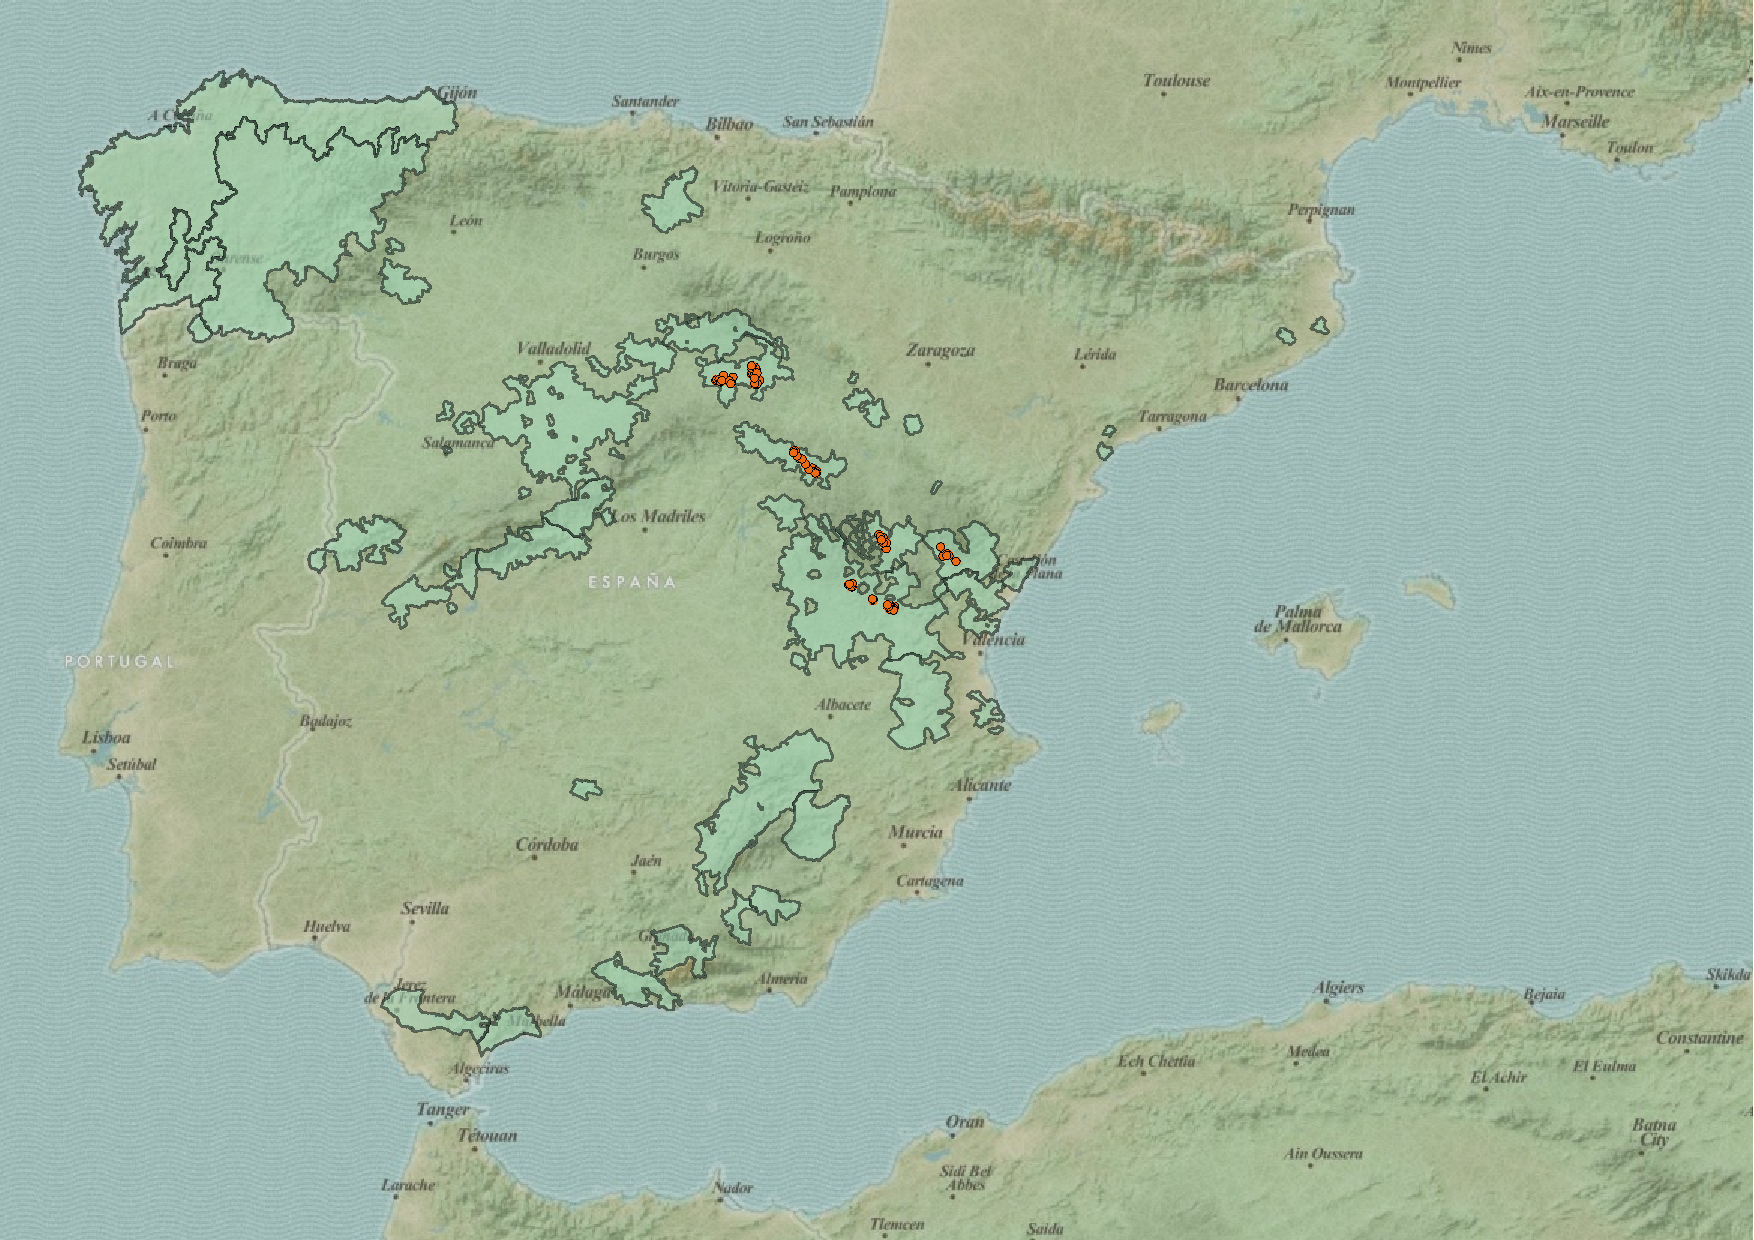
\includegraphics[scale=0.5,trim=20mm 0mm 20mm 0mm]{map_03} 
\caption{Study site. The green areas represent distribution of
  \textit{P. pinaster} along Spain. The orange points represent
  locations of tree-ring chronologies only}
\label{fig:map_03} 
\end{figure}

\clearpage
\begin{figure}\centering
\includegraphics[scale=0.7,trim=20mm 0mm 20mm 0mm]{RWIs} 
\caption{Tree-ring-width chronologies of \textit{P. pinaster} trees
  growing on north (upper-panel plots) and east-central Spain
  (lower-panel plots). Trends in original chronologies (left-panel
  plots) are subtracted (right-panel plots). Gray lines indicate
  fluctuations, and red lines suggest average patterns. Sample depth
  is the number of series available in each year.}
\label{fig:RWIs} 
\end{figure}

\clearpage
\begin{figure}\centering
\includegraphics[scale=0.7,trim=20mm 0mm 20mm 0mm]{ideltas} 
\caption{Isotopic chronologies of \textit{P. pinaster} trees growing
  on north (upper-panel plots) and east-central Spain (lower-panel
  plots). Trends in original chronologies (left-panel plots) are
  subtracted (right-panel plots). Gray lines indicate fluctuations,
  and red lines suggest average patterns. Sample depth is the number
  of series available in each year.}
\label{fig:RWIs} 
\end{figure}

\clearpage
% obn: cambiar south by east-central Spain
\begin{landscape}
\begin{figure}
% \centering
\begin{minipage}[b]{0.8\textwidth}
\centering
\includegraphics[width = \textwidth]{GrowthFunRes}
\end{minipage}
\begin{minipage}[b]{0.8\textwidth}
\includegraphics[width = \textwidth]{IsoFunRes}
\end{minipage}
\label{fig:FunRes}
\caption{Intra-annual response coefficients for precipitation and
  temperature for tree-ring and isotopic chronologies of
  \textit{P. pinaster}. The darker bars indicate signifficant
  coefficients ($P\le0.05$), and the lines represent $95\%$-confidence
  intervals.}
  \end{figure}
\end{landscape}

\clearpage
\begin{figure}
\centering
\includegraphics[scale=0.7,trim=20mm 0mm 20mm 0mm]{coherence1}
\label{fig:coherence1}
\caption{Wavelet coherency between signals of tree-ring widths and
  standardized precipitation indexes. The colored scale indicate the
  correlation between the two time series.}
\end{figure}


% \clearpage
% \begin{figure}\centering
% \includegraphics[scale=0.8,trim=20mm 0mm 20mm 0mm]{clust} 
% \caption{Relative geographic closeness between sample plots. Plots with
%   master series are indicated with m\_. Codes of sample plots begin with
%   initial letter of the species (\textit{P. pinaster}); following with
%   two digits in code indicating the province code: 42 corresponding to
%   \textit{Soria} on Northern protion of \textit{Ebro} river basin, and
%   16 being \textit{Cuenca} on Southern region of such a basin; last
%   three digits in codes indicate individual number of the sample
%   plot. Sample plots of master series have been indicated with the
%   letter m\_. Black dashed line splits distance dendrogram in the two
%   geographical portions of the river basin: North and South (distances
%   $>$ 1500 km); and the red dashed line defines four groups used to
%   statistically control (cross-dating) dendrochronological series
%   (distances $<$ 80 km).}
% \label{fig:clust} 
% \end{figure}

% \clearpage
% \begin{figure}\centering
% \includegraphics[scale=0.8,trim=20mm 0mm 20mm 0mm]{spis} 
% \caption{Series of standardized precipitation indexes (spi) on ten
%   sample plots of \textit{P. pinaster} located on Northern protion of
%   \textit{Ebro} river basin (42: \textit{Soria}) and on Southern
%   region of such a basin (16: \textit{Cuenca}). Panels are ordered
%   from plots with lower spi values (lower-left panel) to plots with
%   higher spi extremes (higher-right panel).See legend in Figure
%   \ref{fig:clust} for further explanation of both: codes and plot
%   locations.}
% \label{fig:spis} 
% \end{figure}

% \clearpage
% \begin{figure}\centering
% \includegraphics[scale=0.9,trim=20mm 0mm 20mm 0mm]{isoYr}
% \caption{Normalized $\delta^{13}$C of
%   \textit{P. pinaster} late-wood in trees growing on Northern Ebro basin
%   (P42) and Southern portion of the basin (P16), Spain}
% \label{fig:isoyr} 
% \end{figure}

 
% \clearpage
% \begin{figure}\centering
% \includegraphics[scale=0.9,trim=20mm 0mm 20mm 0mm]{mflucJun} 
% \caption{Signatures between normalized $\delta^{13}$C of
%   \textit{P. pinaster} late-wood and precipitation indexes
%   (June) from 1974 to 2010. Signatures where computed with Multilevel
%   correlograms. The Fluctuation lags where computed with Sturdges'
%   rule. $10^4$ permutation texts where developed on compared
%   fluctuation-distance matrices.}
% \label{fig:signjun} 
% \end{figure}
% \begin{figure}\centering
% \includegraphics[scale=0.8,trim=20mm 0mm 20mm 0mm]{mflucAug} 
% \caption{Signatures between normalized $\delta^{13}$C of
%   \textit{P. pinaster} late-wood and precipitation indexes
%   (August) from 1974 to 2010. Signatures where computed with Multilevel
%   correlograms. The Fluctuation lags where computed with Sturdges'
%   rule. $10^4$ permutation texts where developed on compared
%   fluctuation-distance matrices.}
% \label{fig:sigaug} 
% \end{figure}

\end{document}
